\documentclass[10.5pt]{article} 
\usepackage[utf8]{inputenc}   
\usepackage[english]{babel}  
\usepackage{amsmath}   
\usepackage{ amssymb }
\usepackage{amsfonts}         
\usepackage{geometry}          
\usepackage{graphicx}
\usepackage{float}
\usepackage{xcolor}
\usepackage{ulem}
\usepackage{tcolorbox}
\usepackage{cancel} 
\usepackage{tikz}
\usepackage{framed}
\usepackage{mdframed}
\usepackage{listings}
\usepackage{xcolor}


\usepackage{parskip} 

\setlength{\parskip}{8pt plus 2pt minus 1pt} 
\setlength{\parindent}{0pt} 

\usepackage{xparse}

\geometry{a4paper, margin=1in} 

\title{Concorde Sonic Boom Simulation. Milestones.}    
\author{César Vidal Fernández}      
\date{17/11/2026}                  

\definecolor{ejercicio}{RGB}{59, 88, 102}
\definecolor{explicacion}{rgb}{0.008, 0.161, 0.098}

\newcommand{\tachareq}[1]{\textcolor{black}{\cancel{#1}}} % Para ecuaciones
\newcommand{\dvt}[1]{\;\mathrm{d}#1}
\newcommand{\separation}{\vspace{10px} \rule{\textwidth}{0.6pt} \par}
\newcommand{\lagrangian}{\mathcal{L}}
\newcommand{\ejercicio}[1]{\color{ejercicio}\textbf{\uline{#1}}\color{black}}
\newcommand{\explicacion}[1]{\color{explicacion}\textit{#1}\color{black}}

\newenvironment{sideline}
{\begin{mdframed}[
		linewidth=1pt,
		topline=false,
		bottomline=false,
		rightline=false,
		leftline=true,
		leftmargin=0cm,
		rightmargin=0cm,
		innertopmargin=0.5cm,
		innerbottommargin=0.5cm
		]}
	{\end{mdframed}}
	
\lstdefinestyle{pythonStyle}{
	language=Python,
	basicstyle=\ttfamily\small,       
	keywordstyle=\color{blue}\bfseries,
	commentstyle=\color{gray}\itshape,  
	stringstyle=\color{teal},           
	numberstyle=\tiny\color{gray},      
	numbers=left,                       
	stepnumber=1,
	numbersep=8pt,
	showstringspaces=false,             
	breaklines=true,                    
	frame=single,                       
	rulecolor=\color{lightgray},        
	tabsize=4
}

% Aplicar este estilo por defecto para los bloques de código
\lstset{style=pythonStyle}

\begin{document}
	
	\maketitle	
	\newpage
	
	\tableofcontents
	\newpage
	
	\section{Sound Engine. First Steps (17/11/2025)}
	
	The first and most important step of the simulation is to create a stable sound that runs smoothly and builds the specific tools that I need. 
	
	For this first day of coding, I decided to implement a basic class with some utility methods that are going to be needed in a daily basis. I didn't want to re-invent the wheel so I decided to call this class Sound().
	
	This class has some attributes that are initialized by default to the following values:
	\begin{itemize}
		\item samplerate: 44000
		\item blocksize: 256
		\item channels: 2 (stereo)
		\item device: None (default output device). This probably be changed in the future, to force the usage of WASAPI.
	\end{itemize}  
	
	And the aforementioned basic methods were created:
	
	\begin{lstlisting}
class Sound():

	def __init__(self, samplerate=44100, blocksize=256, channels=2, device=None):
		self.samplerate = samplerate
		self.blocksize = blocksize
		self.channels = channels
		self.device = device
	
	def to_array(self, path):
		if not os.path.exists(path): return False
		data, file_sr = sf.read(path, dtype="float32", always_2d=True)
		return data, file_sr
	
	def to_mono(self, array):
		if(array.ndim > 1):
		array = np.mean(array, axis=1)
		return array
	
	def play_mp3(self, path):
	
		if not os.path.exists(path): return False
		data, file_sr = self.to_array(path)
	
		sd.play(data, samplerate=file_sr, device=self.device, blocksize=self.blocksize)
		sd.wait()
		return True
	
	def play_array(self, array):
		sd.play(array)
		sd.wait()
		return True
	\end{lstlisting}
	
	\subsection{Generation of White Noise.}
	
	As established in the declaration document, all sounds in the simulation must be created starting using white noise. I created a simple function that pulls random values from a normal distribution in order to build the sound:
	
	\begin{lstlisting}
def generate_white_noise(self, durationSeconds, mean = 0, std_deviation = 0.1):
	if durationSeconds <= 0: return False
	
	num_samples = int(self.samplerate * durationSeconds)
	
	# Generate the values using a normal distribution.
	array = np.random.normal(mean, std_deviation, num_samples)
	return array	
	\end{lstlisting}
	
	\subsection{PSD comparison to the Concorde Motor.}
	
	I searched a video on Youtube of the Concorde flying over a neighborhood in Heathrow. I cut it to an approximated duration of 3 seconds, containing the loudest moments of the video.
	
	For now, we will shape our white noise using only this video. As the project gets bigger, I will try to search more audio examples, recorded from different angles and perspectives, to be able to deduce a variation in sound based on the distance.
	
	To make this comparison we used the Welch's method, included in the scipy.signal library. It computes an estimate of the power spectral density by diving the data into overlapping segments, computing a periodogram\footnote{A Periodogram identifies the dominant frequencies of a signal. It is obtained using the Fourier Fast Transform.} for each segment and averaging them. 
	
	\begin{lstlisting}
def compare_psd(self, first_array, second_array):

	first_array = np.asarray(first_array)
	second_array = np.asarray(second_array)
	
	# Convert to mono arrays
	first_array = self.to_mono(first_array)
	second_array = self.to_mono(second_array)
	
	# Calculate the PSD using the Welch method.
	first_freq, first_density   = sp.signal.welch(first_array, self.samplerate, nperseg=4096)
	second_freq, second_density = sp.signal.welch(second_array, self.samplerate, nperseg=4096)
	
	# Convert to DB to see a more readable scale. Add a small epsilon to avoid zeros in the logarithm.
	first_db = 10 * np.log10(first_density + 1e-10)
	second_db = 10 * np.log10(second_density + 1e-10)
	
	# --- GRAPH ---- # 
	plt.figure(figsize=(12, 6))
	
	plt.plot(first_freq, first_db, label = "First Array", color="blue")
	plt.plot(second_freq, second_db, label = "Second Array", color="red")
	
	plt.title("Comparative PSD response.")
	plt.xlabel("Frequency (Hz)")
	plt.ylabel("Intensity (DB)")
	
	# Center around the audible spectrum.
	plt.xlim(0, 20000)
	
	plt.show()
	\end{lstlisting}	
	
	\begin{figure}[H]
		\centering
		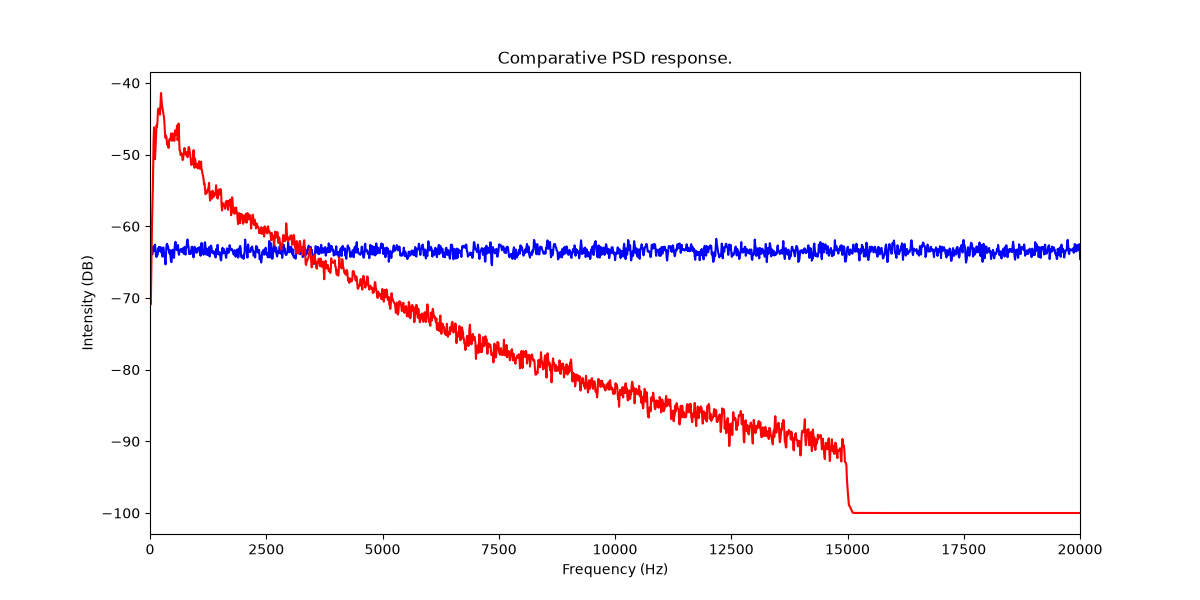
\includegraphics[width=\textwidth]{imgs/first_psd.png}
	\end{figure}
	
	From this information, we can obtain to clear conclusions: 
	\begin{itemize}
		\item The motor concentrates its sound intensity between 20 to 3000Hz, it linearly fades until 15000hz, where it completely disappears. 
		
		\item The absence of sound above 15kHz can be justified with poor recording quality or aggressive compression methods. I will ignore this cap and make a linear descent to 20kHz. 
	\end{itemize}
	
	
	
	
	 
	
\end{document}
